\documentclass[a4paper]{article}
\usepackage[14pt]{extsizes} 
\usepackage[T2A]{fontenc}
\usepackage[utf8]{inputenc}
\usepackage{natbib}
\usepackage{graphicx}
\usepackage{amsmath}
\usepackage[english]{babel}
\usepackage{fontspec}
\usepackage{amsmath,amsfonts,amssymb,amsthm,mathtools,mathrsfs}
\usepackage{icomma}
\usepackage{fullpage}
\usepackage{ulem}
\usepackage{eufrak}
\usepackage{setspace}
\usepackage{listings}
\usepackage{indentfirst}
\usepackage[left=2cm,right=1.5cm,top=2cm,bottom=2cm]{geometry}
\usepackage{xcolor}
\usepackage{float}
\usepackage{csquotes}

\setmainfont[Ligatures={TeX,Historic}]{Times New Roman}
\setlength{\parindent}{5ex}
\setlength{\parskip}{1em}
\renewcommand{\baselinestretch}{1}

\graphicspath{{images/}}

\definecolor{buzzlightyear}{HTML}{8757A5}
\definecolor{grass}{HTML}{738D06}
\definecolor{literal}{HTML}{F18A2B}
\definecolor{commentcolor}{HTML}{8E908B}

\lstdefinestyle{habrstyle}{
    backgroundcolor=\color{white},   
    commentstyle=\color{commentcolor},
    keywordstyle=\bfseries\color{buzzlightyear},
    numberstyle=\tiny\color{commentcolor},
    stringstyle=\color{grass},
    basicstyle=\ttfamily\footnotesize,
    breakatwhitespace=false,         
    breaklines=true,                 
    captionpos=b,                    
    keepspaces=true,                 
    numbers=left,                    
    numbersep=5pt,                  
    showspaces=false,                
    showstringspaces=false,
    showtabs=false,                  
    tabsize=4
}

\lstset{style=habrstyle}

\begin{document}

    % FIRST PAGE
    \begin{center}
        \begin{center}
        \hfill \break
        \normalsize{Санкт-Петербургский государственный политехнический}\\
        \normalsize{университет Петра Великого}\\
        \hfill \break
        \normalsize{\textbf{Высшая школа интеллектуальных систем и}}\\ 
        \normalsize{\textbf{суперкомпьютерных технологий}}\\ 
        \hfill \break
        \hfill \break
        \hfill \break
        \normalsize{Лабораторная работа}\\
        \hfill \break
        \hfill \break
        \normalsize{\LARGE Дифференцирование и интегрирование}\\
        \end{center}
        \hfill \break
        \hfill \break
        \hfill \break
        \hfill \break
        \hfill \break
        \hfill \break
        \hfill \break
        \hfill \break
        \hfill \break
        \hfill \break
        \begin{flushright}
            \normalsize{Работу выполнил студент}\\
            \normalsize{3-го курса, группа 3530901/80201}\\
            \normalsize{Сахибгареев Рамис Ринатович}\\
            \hfill \break
            \normalsize{Преподаватель:}\\
            \normalsize{Богач Наталья Владимировна}\\
        \end{flushright}
        \hfill \break
        \hfill \break
        \hfill \break
        \hfill \break
        \begin{center} Санкт-Петербург 2021 \end{center}
        \thispagestyle{empty}
    \end{center}
    % FIRST PAGE [END]
    
    \newpage
        \tableofcontents
    
    \newpage
         \listoffigures
    
    \newpage
         \lstlistoflistings   
     
    % START START START START START
    \newpage
        \section{Part 1: Research and execution of chap08}
        
        In this part we need to research and execute existing chap09.ipynb file, that contains information about derivative and integral filters.
        
        Difference is an analogue for derivative and it acts like high-pass filter. Cumulative sum is a analogue of integral and it acts like low-pass filter.
        
        \begin{figure}[H]
            \centering
            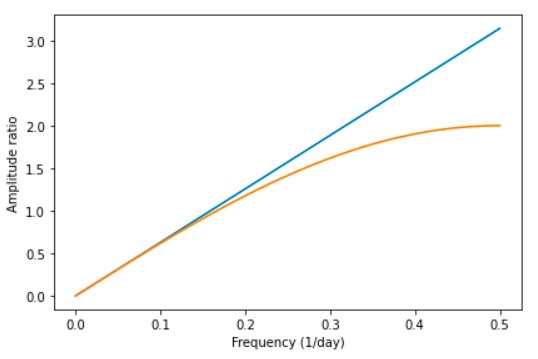
\includegraphics[width=\textwidth]{img/p1_1.png}
            \caption{Diff and deriv fitlers}
            \label{fig:p1_2}
        \end{figure}
        
        \begin{figure}[H]
            \centering
            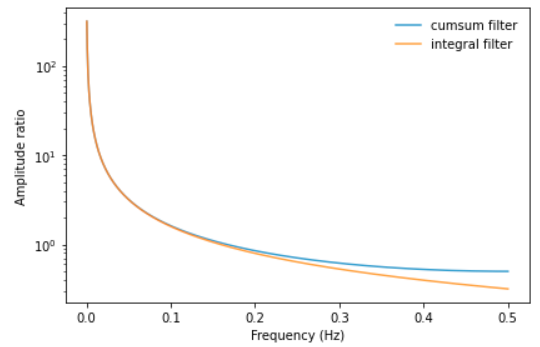
\includegraphics[width=\textwidth]{img/p1_2.png}
            \caption{Cumsum and integral filters}
            \label{fig:p1_2}
        \end{figure}
        
        But convolution theorem works only for periodic signals, that's why trying to apply cumsum/integral filter on the non periodic signal results wrong result.
        
        \begin{figure}[H]
            \centering
            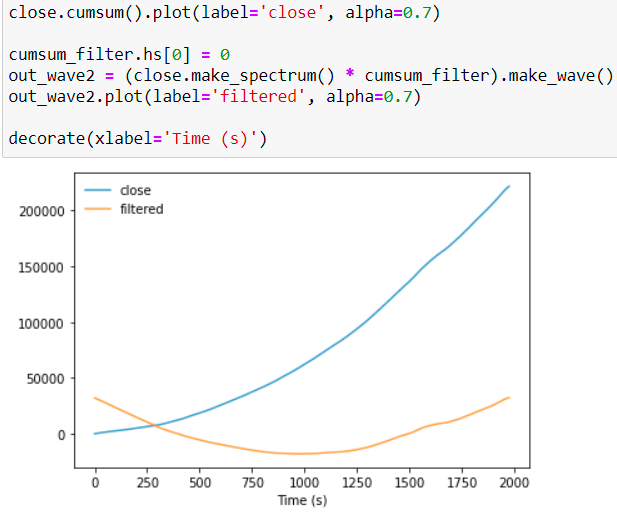
\includegraphics[width=\textwidth]{img/p1_3.png}
            \caption{Trying to apply convolution theorem on non periodic signal}
            \label{fig:p1_1}
        \end{figure}
        
    \newpage
        \section{Part 2: Diff on wave and on its spectrum}

        In this part we need to compare diff calculation result on the wave and on its spectrum.
        For test triangle signal was used.
        
        \begin{lstlisting}[language=Python,caption=Diff and deriv code,label={lst:part1_2}]
    import numpy as np
    import matplotlib as plt
    from thinkdsp import *
    
    wave = TriangleSignal(freq=50).make_wave(duration=0.1, framerate=44100)
    wave.plot()
    decorate(xlabel='Time (s)')
    
    wave_diff = wave.diff()
    wave_diff.plot()
    decorate(xlabel='Time (s)')
    
    wave.make_spectrum().differentiate().make_wave().plot()
    decorate(xlabel='Time (s)')
        \end{lstlisting}
        
        \begin{figure}[H]
            \centering
            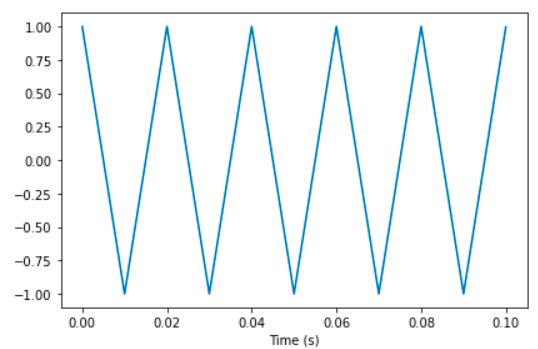
\includegraphics[width=\textwidth]{img/p2_1.png}
            \caption{Triangle wave}
            \label{fig:part1_1_2}
        \end{figure}
        
        \begin{figure}[H]
            \centering
            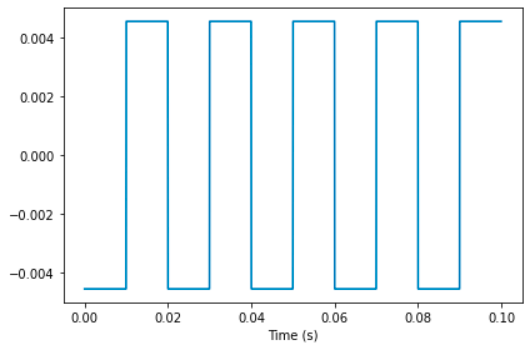
\includegraphics[width=\textwidth]{img/p2_2.png}
            \caption{Triangle wave's diff}
            \label{fig:part1_1_2}
        \end{figure}
        
        \begin{figure}[H]
            \centering
            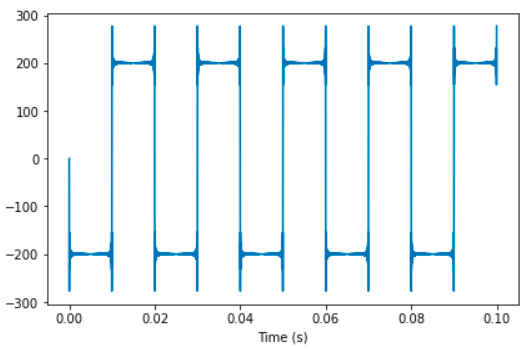
\includegraphics[width=\textwidth]{img/p2_3.png}
            \caption{Spectrum's diff}
            \label{fig:part1_1_2}
        \end{figure}
        
        We can see, that diff of a triangle signal is a square signal. However, applying diff on the spectrogram results something like square signal, but with peaks on the edges of the squares. It happens because we cannot differentiate triangle signal on the edge points.
            
    \newpage
        \section{Part 3: Cumsum and integrate}
        
        In this part, we need to compare cumsum and integrate. To do it we can use diff result from the previous part, trying to restore original signal.
            
        \begin{lstlisting}[language=Python,caption=Integration code,label={lst:part1_2}]
    wave_sum = wave_diff.cumsum()
    wave_sum.unbias()
    spec_int = wave_diff.make_spectrum().integrate()
    spec_int.hs[0] = 0
    wave_int = spec_int.make_wave()
    wave_int.normalize()
    wave_sum.plot()
    wave_int.plot()
        \end{lstlisting}
        
        \begin{figure}[H]
            \centering
            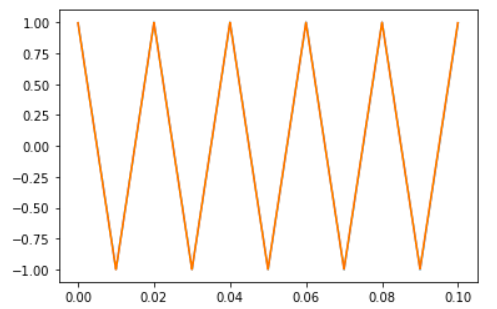
\includegraphics[width=\textwidth]{img/p3_1.png}
            \caption{Restore result}
            \label{fig:part1_1_2}
        \end{figure}
        
        We can see, that they both restored signal successful and absolutely same. However, for cumsum we need to perform unbias, and for integral we need to set hs[0] as well as normalize the result.
        
    \newpage
        \section{Part 4: Double integration}
        
        In this part, we need to perform double cumsum and integration using sawtooth signal.
            
        \begin{lstlisting}[language=Python,caption=Double integration,label={lst:part1_2}]
    wave = SawtoothSignal(freq=50).make_wave(duration=0.1, framerate=44100)
    wave.plot()
    decorate(xlabel='Time (s)')
    wave_sum = wave.cumsum()
    wave_sum.unbias()
    wave_sum = wave_sum.cumsum()
    wave_sum.plot()
    spec_int = wave.make_spectrum().integrate().integrate()
    spec_int.hs[0] = 0
    wave_int = spec_int.make_wave()
    wave_int.plot()
    wave_int.make_spectrum().plot()
    plt.xlim(left=0, right=500)
        \end{lstlisting}
        
        \begin{figure}[H]
            \centering
            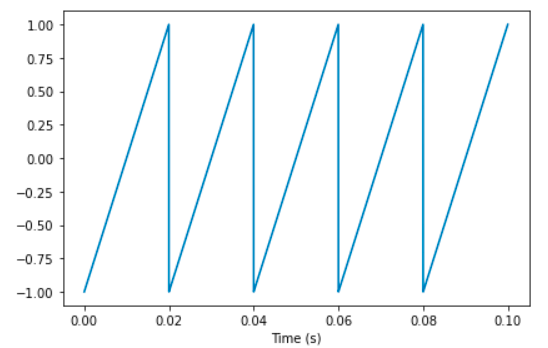
\includegraphics[width=\textwidth]{img/p4_1.png}
            \caption{Sawtooth signal to be integrated}
            \label{fig:part1_1_2}
        \end{figure}

        After applying cumsum and integration we got next results:
        
        \begin{figure}[H]
            \centering
            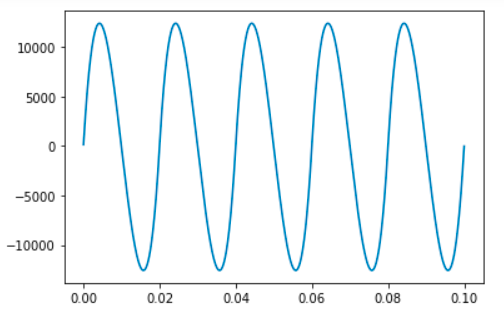
\includegraphics[width=\textwidth]{img/p4_2.png}
            \caption{Cumsum result}
            \label{fig:part1_1_2}
        \end{figure}
        
        \begin{figure}[H]
            \centering
            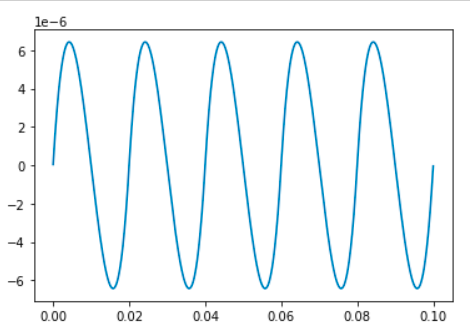
\includegraphics[width=\textwidth]{img/p4_3.png}
            \caption{Integration result}
            \label{fig:part1_1_2}
        \end{figure}
        
        We can see, that there are no differences between two methods. Signal looks like sin signal, but it is a cubic signal. The reason it happens is that integration acts like low pass filter, so only fundamental frequency has most of signals power.
        
        \begin{figure}[H]
            \centering
            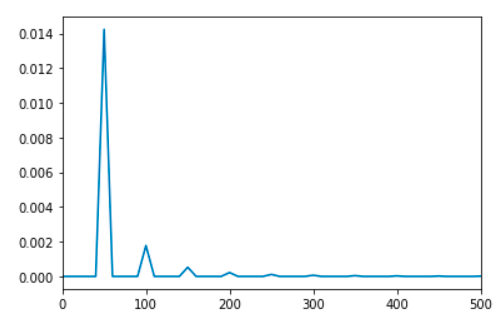
\includegraphics[width=\textwidth]{img/p4_4.png}
            \caption{Integration spectrum}
            \label{fig:part1_1_2}
        \end{figure}
        
    \newpage
        \section{Part 5: Double differentiate}
        
        In this part, we need to perform double diff and derivative using cubic signal. It is good to have framerate = 1, because that way filters will be same scale.
            
        \begin{lstlisting}[language=Python,caption=Double diff,label={lst:part1_2}]
    wave = CubicSignal(freq=0.0005).make_wave(duration=10000, framerate=1)
    wave.plot()
    
    wave_diff = wave.diff().diff()
    wave_diff.plot()
    
    wave_der = wave.make_spectrum().differentiate().differentiate().make_wave()
    wave_der.plot()
    
    diff_window = np.array([-1.0, 2.0, -1.0])
    padded = zero_pad(diff_window, len(wave))
    diff_wave = Wave(padded, framerate=wave.framerate)
    diff_filter = diff_wave.make_spectrum()
    diff_filter.plot(label='2nd diff')
    decorate(xlabel='Frequency (Hz)', ylabel='Amplitude ratio')
    
    deriv_filter = wave.make_spectrum()
    deriv_filter.hs = (np.pi * 2 * 1j * deriv_filter.fs)**2
    deriv_filter.plot(label='2nd deriv')
    decorate(xlabel='Frequency (Hz)', ylabel='Amplitude ratio')
        \end{lstlisting}
        
        \begin{figure}[H]
            \centering
            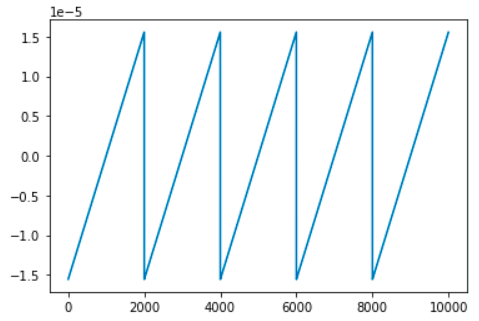
\includegraphics[width=\textwidth]{img/p5_1.png}
            \caption{Diff result}
            \label{fig:part1_1_2}
        \end{figure}
        
        \begin{figure}[H]
            \centering
            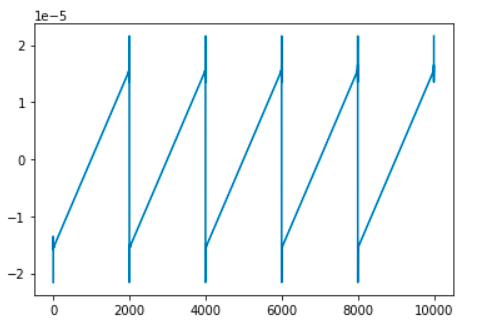
\includegraphics[width=\textwidth]{img/p5_2.png}
            \caption{Deriv result}
            \label{fig:part1_1_2}
        \end{figure}
        
        We can see, that wave differentiation results a clear sawtooth signal. Spectrum differentiation, on the other hand, also results a sawtooth signal, but it has spikes on the edges. It happens because parabolic signal, that we got on the first diff, has some points, that cannot be differentiated.
        
        \begin{figure}[H]
            \centering
            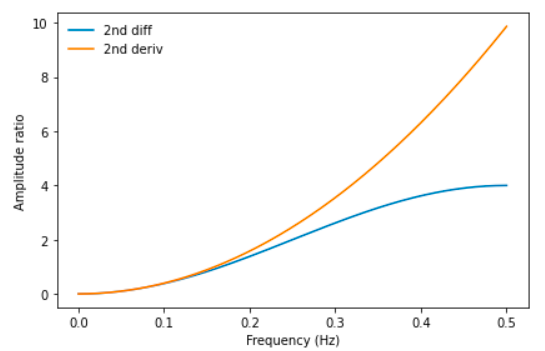
\includegraphics[width=\textwidth]{img/p5_3.png}
            \caption{Comparing filters}
            \label{fig:part1_1_2}
        \end{figure}.
        
        For 2nd diff filter is known - [-1 2 -1]. For deriv filter we can simply perform double applying of 1st deriv filter. We see, that trend continues - deriv filter is more exponential, while diff filter has fast rice on the low frequencies and slows down on the high frequencies. That's why they acts same on the low frequencies, but differs on the high frequencits.
            
    \newpage
        \section{Conclusion}
            We've learned, how cumulutive sum, integration, diff and deriv affects the signal. Integration and cumulative sum acts like a low pass filter, while diff and deriv acts like a high pass filter. Because they are opposites, we can convert signal into different forms using this operations, also restoring the signals. However, due to loss of an information during differentiation procedure, we cannot restore signal fully.
     
\end{document}
